\documentclass{beamer}\usepackage[]{graphicx}\usepackage[]{color}
%% maxwidth is the original width if it is less than linewidth
%% otherwise use linewidth (to make sure the graphics do not exceed the margin)
\makeatletter
\def\maxwidth{ %
  \ifdim\Gin@nat@width>\linewidth
    \linewidth
  \else
    \Gin@nat@width
  \fi
}
\makeatother

\definecolor{fgcolor}{rgb}{0.345, 0.345, 0.345}
\newcommand{\hlnum}[1]{\textcolor[rgb]{0.686,0.059,0.569}{#1}}%
\newcommand{\hlstr}[1]{\textcolor[rgb]{0.192,0.494,0.8}{#1}}%
\newcommand{\hlcom}[1]{\textcolor[rgb]{0.678,0.584,0.686}{\textit{#1}}}%
\newcommand{\hlopt}[1]{\textcolor[rgb]{0,0,0}{#1}}%
\newcommand{\hlstd}[1]{\textcolor[rgb]{0.345,0.345,0.345}{#1}}%
\newcommand{\hlkwa}[1]{\textcolor[rgb]{0.161,0.373,0.58}{\textbf{#1}}}%
\newcommand{\hlkwb}[1]{\textcolor[rgb]{0.69,0.353,0.396}{#1}}%
\newcommand{\hlkwc}[1]{\textcolor[rgb]{0.333,0.667,0.333}{#1}}%
\newcommand{\hlkwd}[1]{\textcolor[rgb]{0.737,0.353,0.396}{\textbf{#1}}}%
\let\hlipl\hlkwb

\usepackage{framed}
\makeatletter
\newenvironment{kframe}{%
 \def\at@end@of@kframe{}%
 \ifinner\ifhmode%
  \def\at@end@of@kframe{\end{minipage}}%
  \begin{minipage}{\columnwidth}%
 \fi\fi%
 \def\FrameCommand##1{\hskip\@totalleftmargin \hskip-\fboxsep
 \colorbox{shadecolor}{##1}\hskip-\fboxsep
     % There is no \\@totalrightmargin, so:
     \hskip-\linewidth \hskip-\@totalleftmargin \hskip\columnwidth}%
 \MakeFramed {\advance\hsize-\width
   \@totalleftmargin\z@ \linewidth\hsize
   \@setminipage}}%
 {\par\unskip\endMakeFramed%
 \at@end@of@kframe}
\makeatother

\definecolor{shadecolor}{rgb}{.97, .97, .97}
\definecolor{messagecolor}{rgb}{0, 0, 0}
\definecolor{warningcolor}{rgb}{1, 0, 1}
\definecolor{errorcolor}{rgb}{1, 0, 0}
\newenvironment{knitrout}{}{} % an empty environment to be redefined in TeX

\usepackage{alltt}
\IfFileExists{upquote.sty}{\usepackage{upquote}}{}
\begin{document}

%' #' <<preparation, echo=FALSE>>=
%' #' ## Da war ich schon
%' #' places_visited <- c("Berlin", "San Francisco", "Leiden", "Eindhoven", 
%' #'                     "Innsbruck", "Munich", "Palo Alto", "La Spezia", "Elba", 
%' #'                     "Barcelona", "Lombock", "Bali", "Singapore", "Beijing",
%' #'                     "Shanghai", "Osaka", "Tokyo")
%' #' 
%' #' ## Wo auf der Welt sind diese Orte?
%' #' library("ggmap")
%' #' lonlat <- geocode(places_visited) 
%' #' lonlat
%' #' my_visits <- data.frame(city = places_visited, lonlat)
%' #' my_visits
%' #' 
%' #' save(my_visits, file = "urlaub.rda")
%' #' @


\begin{frame}
\begin{columns}
  \column{0.3\textwidth}
  
\includegraphics[width=\textwidth]{me}
  
  \column{0.7\textwidth}
  \visible<2->{
\includegraphics[width=\textwidth]{formel}}\\[2em]
  \visible<3->{
\includegraphics[width=\textwidth]{frage_antwort1}}\\[2em]
  % \only<4>{
\includegraphics[width=\textwidth]{herz}}
  \visible<4>{
\includegraphics[width=\textwidth]{herz1}}
\end{columns}
\end{frame}


\begin{frame}[fragile]{}
\begin{knitrout}
\definecolor{shadecolor}{rgb}{0.969, 0.969, 0.969}\color{fgcolor}
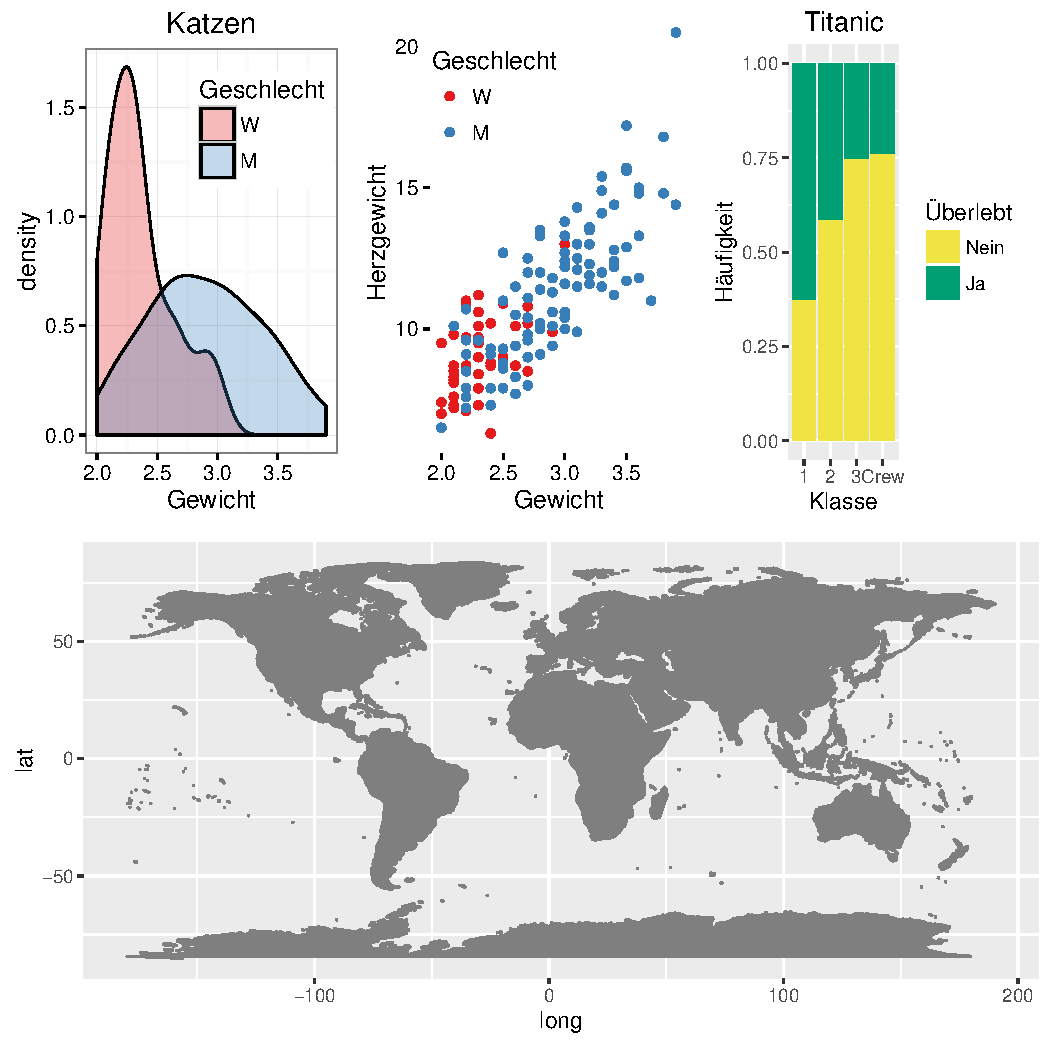
\includegraphics[width=\maxwidth,height=\textheight]{figure/graphiken-1} 

\end{knitrout}
\end{frame}



\begin{frame}[fragile]{Wie geht das?}
\small
\begin{knitrout}
\definecolor{shadecolor}{rgb}{0.969, 0.969, 0.969}\color{fgcolor}\begin{kframe}
\begin{alltt}
\hlkwd{library}\hlstd{(}\hlstr{"ggplot2"}\hlstd{)}
\hlstd{karte} \hlkwb{<-} \hlkwd{ggplot}\hlstd{()} \hlopt{+}
  \hlkwd{borders}\hlstd{(}\hlstr{"world"}\hlstd{,} \hlkwc{colour}\hlstd{=}\hlstr{"gray50"}\hlstd{,} \hlkwc{fill}\hlstd{=}\hlstr{"gray50"}\hlstd{)} \hlopt{+}
  \hlkwd{coord_quickmap}\hlstd{()}
\hlstd{karte}
\end{alltt}
\end{kframe}
\end{knitrout}
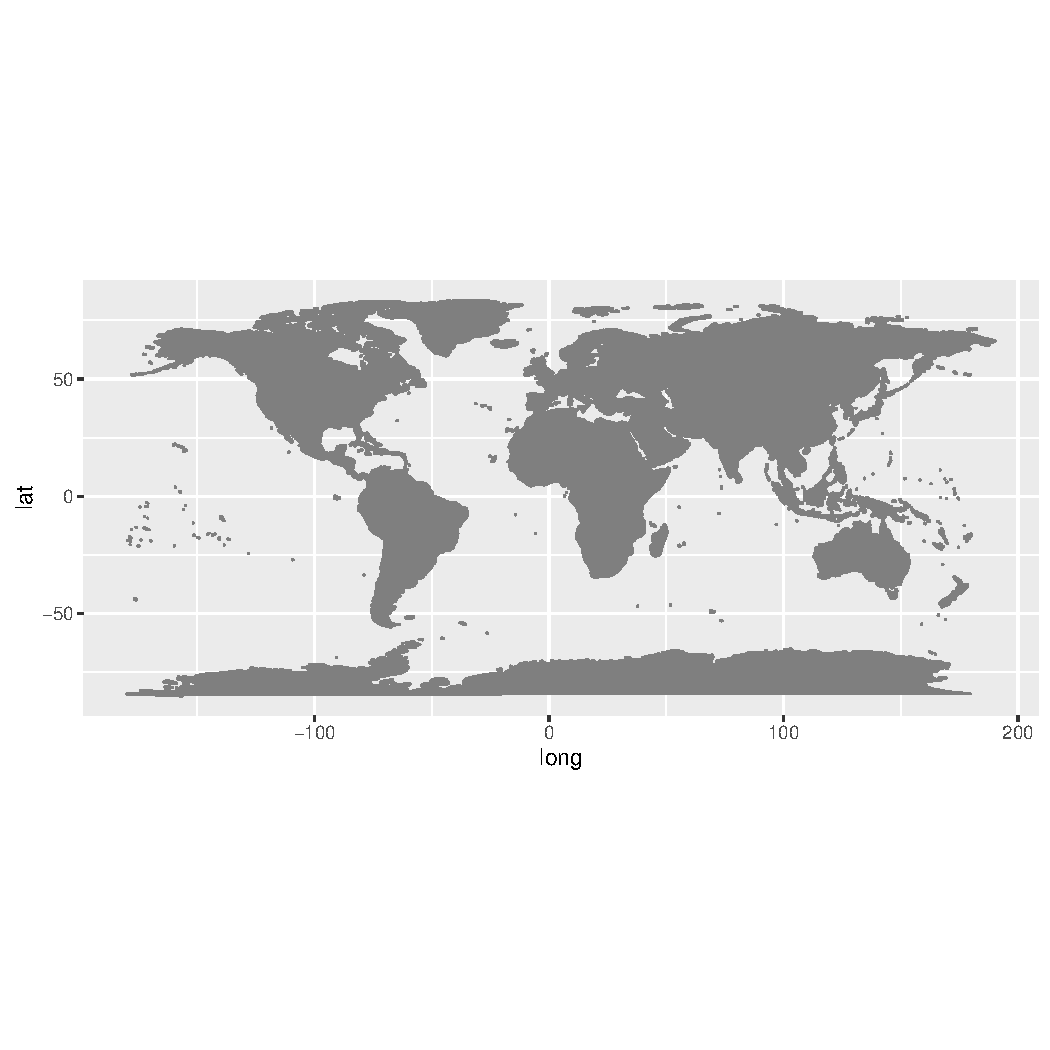
\includegraphics[width = \textwidth, trim={0 13em 0em 13em}, clip]{figure/karte-1}
\end{frame}


\begin{frame}[fragile]{Heidis Urlaube}
\small
\begin{knitrout}
\definecolor{shadecolor}{rgb}{0.969, 0.969, 0.969}\color{fgcolor}\begin{kframe}
\begin{alltt}
\hlkwd{load}\hlstd{(}\hlstr{"urlaub.rda"}\hlstd{)}
\hlstd{karte_urlaub} \hlkwb{<-} \hlstd{karte} \hlopt{+}
  \hlkwd{geom_point}\hlstd{(}\hlkwc{data} \hlstd{= my_visits,} \hlkwd{aes}\hlstd{(}\hlkwc{x} \hlstd{= lon,} \hlkwc{y} \hlstd{= lat))}
\hlstd{karte_urlaub}
\end{alltt}
\end{kframe}
\end{knitrout}
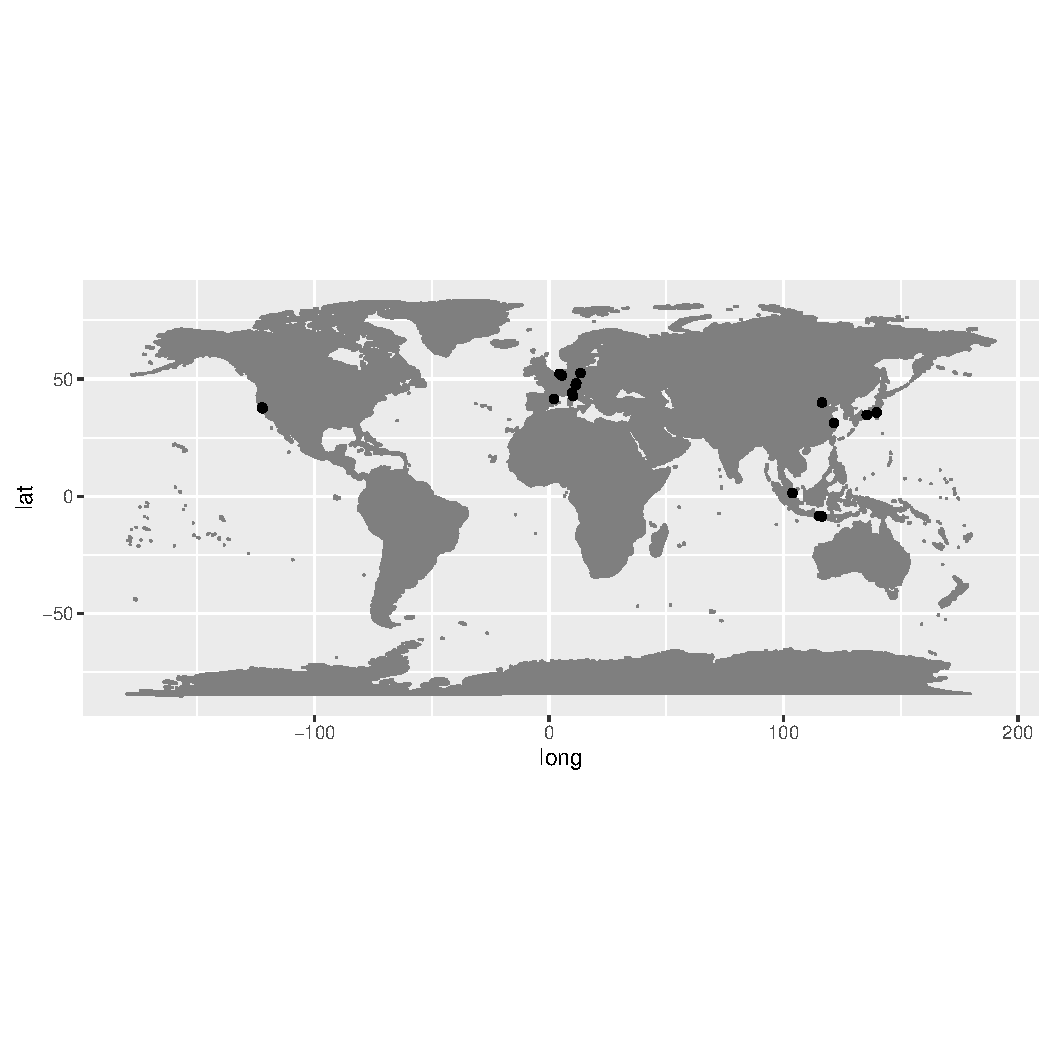
\includegraphics[width = \textwidth, trim={0 10em 0em 10em}, clip]{figure/urlaubskarte-1}
\end{frame}

\end{document}
